\section{Application in equipment selection}
\subsection{Algorithm workflow}
The warehouse facility model is subject to various constraints defined in the previous section, and exact methods like branch-and-bound and mathematical programming take very long time to reach optimal solutions.
On the other hand, metaheuristic algorithms have been successfully applied in many engineering optimization problems.
Bee colony optimization (BCO) is a metaheuristic algorithm that imitates the mating process of bee colonies.
A bee colony consists of four types of bees, namely, queen bee, drone, worker bee and bee larva. 
There usually exist only one queen bee within a colony and it is often the one who lives the longest.
The queen bee aims to mate with drones to produce larvae.
A drone is a haploid that mates with the queen bee and dies after the mating process.
Genes of the drone enter the queen bee and passe along to larvae.
Worker bee exists to produce honey to provide food for larvae, which grow up to be either queen bee or drones.
Abbass proposed a bee colony optimization algorithm based on the observation of a bee colony's mating and reproduce process, and successfully applied it to various engineering optimization problems.


In BCO, bees, including the queen bee, drones and larvae, represent individual solutions to the problem at hand and all the constraints are embedded in the solution representation.
In other words, a bee represents a feasible solution to the warehouse facility location problem depicted by the mathematical model described in the previous section.
In BCO, the number of times that the queen bee mates is determined by the number of drones, the results of the mating process decide the size of larvae.
The size of the queen bee's ovary indicates the storage size of drones' genes.
The number of iterations indicates the number of mating process.
The workflow of BCO can be summarised as follows:
\begin{itemize}
	\item Initialize parameters of the BCO.
	\item Create the initial population and calculate their fitness values. Selected the bee with the best fitness value and use it as the queen bee, the rest bees are used as drones.
	\item Check whether stopping criteria is met, stop if so, go to the next step otherwise.
	\item Initialize the ovary, energy and speed of the queen bee. 
	Repeat the following steps if the energy is bigger than the threshold and ovary is not full: 1) choose a drone and let it mate with the queen been if mating criteria is met, put its genes into the ovary; 2) decrease the energy and speed of the queen bee.
	\item The queen bee selects sequentially the genes in its ovary to produce larvae, which is then raised by different worker bees. If the resulting bee has a better fitness value than the queen bee, it becomes the new queen bee. Similarly it becomes a drone if its fitness value is better than any of the drones.
	\item Output the queen bee.
\end{itemize}



\subsection{Encoding scheme}
This paper uses a integer-based encoding scheme which consists of two parts.
Take the rail transit system of Wuhan as an example, part two of a solution uses a binary value to indicate whether a warehouse facility is chosen at the corresponding rail lane or not, part one of the solution decides the warehouse facility servicing the corresponding rail lane.
Figure \ref{fig:fig1} shows that rail lanes 1, 3, 4, 6, 7, 8 are selected to build warehouse facilities and the eight lanes will be serviced by the warehouse facilities built on lanes 1, 1, 3, 4, 7, 6, 7, 8, respectively.

\begin{figure}[h!]
	\begin{center}
		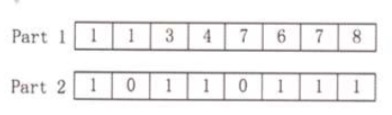
\includegraphics[width=0.5\linewidth]{sections/figure1.jpg}
		\caption{Illustration of the encoding scheme of warehouse facilities}
		\label{fig:fig1}
	\end{center}
\end{figure}

\subsection{Fitness function}
The fitness value of an individual in the bee colony is indicated by the total cost computed from the underlying solution it represents.
As discussed in earlier section, the cost consists of three components, namely, construction cost, maintenance cost and operational cost:
\begin{align}
	F_{fitness} = M - (C_1 + C_2 + C_3)
\end{align}
where $F_{fitness}$ is the fitness value of a bee in the colony, and it is computed using the three cost components.
Note that $M$ is a big number and the more cost a solution takes, the worse its fitness value is.

\subsection{Crossover operator}
This paper uses the single-point crossover operator depicted in figure \ref{fig:fig2}.
In figure \ref{fig:fig2}, two parent bees $P1$ and $P2$ creates a new offspring solution $O1$ through crossover.
The crossover operator involves two steps, focusing on two parts of a solution respectively.
The crossover operation on part two employs a two-point crossover operator.

\begin{figure}[h!]
	\begin{center}
		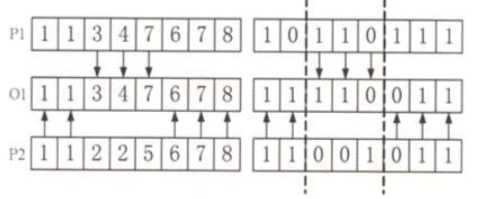
\includegraphics[width=0.5\linewidth]{sections/figure2.jpg}
		\caption{Illustration of the crossover operator}
		\label{fig:fig2}
	\end{center}
\end{figure}

\subsection{Local search algorithm}
The worker bees in the BCO algorithm refer to various local search algorithms that are used to improve the new offspring solutions generated by the crossover operator.
These larvae grow up to be either queen bee or drones and the same larva may grow up into either role if raised by different worker bees.
On the other hand, different larvae may grow up into either role even raised by the same work bees.
This paper uses three different local search heuristics, namely, point insertion, random position swap and adjacent position swap.





